\documentclass[11pt,a4paper]{report}

% ---------- PACKAGES ----------
\usepackage[utf8]{inputenc}
\usepackage[T1]{fontenc}
\usepackage{times}
\usepackage[margin=0.9in]{geometry}
\usepackage{graphicx}
\usepackage{tikz}
\usetikzlibrary{shapes.geometric, arrows.meta, positioning, fit, backgrounds}
\usepackage{booktabs}
\usepackage{array}
\usepackage{fancyhdr}
\usepackage{titlesec}
\usepackage{enumitem}
\usepackage{hyperref}
\usepackage{xcolor}
\usepackage{caption}

\setlist{itemsep=1pt, topsep=3pt, parsep=1pt}

\hypersetup{
    colorlinks=true,
    linkcolor=black,
    citecolor=black,
    urlcolor=blue,
    pdftitle={MedFinder: Real-Time Medicine Availability and Store Locator},
    pdfauthor={Madhav Gupta, Sourabh Chhabra, Arpit Yadav}
}

% ---------- HEADER/FOOTER ----------


\titleformat{\chapter}[display]
  {\normalfont\Large\bfseries}{\chaptertitlename\ \thechapter}{8pt}{\Large}
\titlespacing*{\chapter}{0pt}{-10pt}{10pt}
\titlespacing*{\section}{0pt}{8pt}{4pt}
\titlespacing*{\subsection}{0pt}{6pt}{3pt}

% Colors for diagram boxes
\definecolor{blueBox}{RGB}{198,217,241}
\definecolor{tealBox}{RGB}{198,235,235}
\definecolor{orangeBox}{RGB}{252,228,178}
\definecolor{redBox}{RGB}{248,206,204}
\definecolor{greenBox}{RGB}{198,239,206}

\begin{document}

% ============================================================
% TITLE PAGE
% ============================================================
\begin{titlepage}
    \centering
    \vspace*{0.3cm}
    {\large UCS503 -- Software Engineering Project\par}
    {\large Academic Year 2026--2027\par}
    \vspace{0.8cm}

    
\includegraphics[width=3.5cm]{thapar_logo.png}

    \vspace{0.8cm}

    {\Huge\bfseries MedFinder: Real-Time\par}
    {\Huge\bfseries Medicine Availability \& Store Locator\par}
    \vspace{0.6cm}
    {\Large Dynamic Inventory Search and Store-Level\par}
    {\Large Medicine Reservation Platform\par}

    \vspace{1.5cm}

    {\Large\bfseries Submitted by:\par}
    \vspace{0.6cm}

    \begin{tabular}{@{}ll@{}}
        \textbf{1024030436} & Madhav Gupta \\[0.3cm]
        \textbf{1024030435} & Sourabh Chhabra \\[0.3cm]
        \textbf{1024030446} & Arpit Yadav \\
    \end{tabular}

    \vspace{1cm}
    {\Large B.E. Third Year, Computer Science \& Engineering\par}

    \vfill

    {\Large\bfseries Submitted to:\par}
    \vspace{0.3cm}
    {\Large\bfseries Dr. Jeelani Asif\par}
    \vspace{0.3cm}
    {\large Department of Computer Science and Engineering\par}

    \vspace{0.8cm}
    {\large\bfseries Mid-Semester Evaluation Report\par}
    \vspace{0.8cm}

    {\large Computer Science and Engineering Department\par}
    {\large Thapar Institute of Engineering and Technology, Patiala\par}

\end{titlepage}

% ============================================================
% TABLE OF CONTENTS
% ============================================================
\tableofcontents
\thispagestyle{empty}
\newpage

% ============================================================
% CHAPTER 1: INTRODUCTION
% ============================================================
\chapter{Introduction}

\section{Background and Context}

Access to the right medicine at the right time is a basic requirement of healthcare, yet no medical store stocks every medicine at all times. Patients routinely discover -- only after travelling to a pharmacy -- that the medicine they need is out of stock, unavailable in the required strength, or simply not carried by that store. This is true both for specialised or prescription-only drugs and, at times, for common over-the-counter medicines that have temporarily run out.

This problem becomes especially serious during urgent or emergency situations, and disproportionately affects elderly patients, chronically ill patients, and caregivers who cannot easily visit several pharmacies in sequence. At present there is no simple, centralised way for a patient to check, before leaving home, which nearby recognised pharmacy actually has a given medicine in stock. MedFinder is proposed as a web application that addresses this gap directly: it lets a user search for a medicine and instantly see which verified, nearby pharmacies currently stock it, along with price and distance, so that the user can go straight to a store that can actually fulfil their need.

\subsection{Problem Statement}

Patients lack a centralised, real-time way to know which nearby pharmacy has a required medicine in stock. This leads to wasted time, unnecessary travel, and, in urgent cases, delayed treatment. Even after a patient identifies a store that reportedly has the medicine, there is no guarantee it will still be available by the time they arrive, since stock can be sold out in the interim. This uncertainty affects both rare, specific medicines and everyday medicines alike, and stems fundamentally from the lack of visibility into store-level inventory that patients currently have. MedFinder resolves this gap through a centralised inventory-search system that queries live, store-level stock records and returns a ranked list of verified pharmacies that actually hold the requested medicine.

\section{Project Objectives}

The core objectives of the MedFinder project comprise:

\begin{itemize}
    \item \textbf{Centralised Inventory Listing:} Provide a single platform listing recognised medical stores in a given area along with their live medicine inventory.
    \item \textbf{Search, Filter \& Rank:} Allow users to search for a specific medicine and view results filtered and sorted by nearby distance and lowest price.
    \item \textbf{Travel-Time Reduction:} Reduce the time and travel patients currently spend visiting or calling multiple pharmacies to locate a medicine.
    \item \textbf{Reservation Mechanism:} Offer a Reserve feature so a user can hold a medicine at a chosen store until they arrive, reducing the risk of it selling out in the meantime.
    \item \textbf{Trust \& Verification:} Ensure trust and safety by only listing pharmacies that have gone through a verification/registration process.
    \item \textbf{Scalable Engineering Stack:} Build the system on a reliable, maintainable engineering stack that can scale from a small prototype to a citywide deployment.
\end{itemize}

% ============================================================
% CHAPTER 2: METHODOLOGY AND DESIGN
% ============================================================
\chapter{Methodology and Design}

\section{System Architecture}

\subsection{High-Level Design}

MedFinder follows a standard three-tier web architecture organized into the \textbf{Client Layer}, the \textbf{Application Layer}, and the \textbf{Data Layer}. Figure 2.1 illustrates the high-level architecture.

\begin{figure}[h!]
\centering
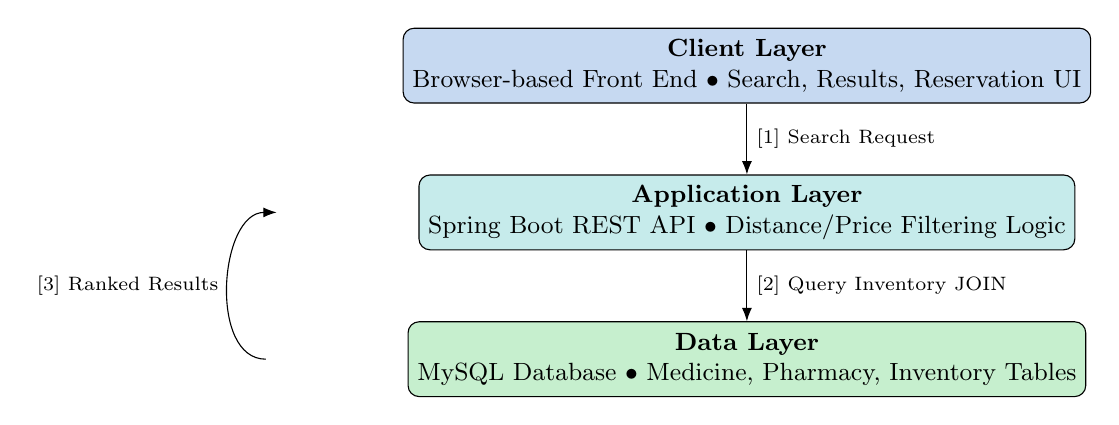
\begin{tikzpicture}[
    box/.style={rectangle, draw, rounded corners, minimum width=8.2cm, minimum height=0.95cm, align=center, font=\small},
    arrowlabel/.style={font=\scriptsize, align=center}
]
\node[box, fill=blueBox] (client) {\textbf{Client Layer} \\ Browser-based Front End $\bullet$ Search, Results, Reservation UI};
\node[box, fill=tealBox, below=0.9cm of client] (app) {\textbf{Application Layer} \\ Spring Boot REST API $\bullet$ Distance/Price Filtering Logic};
\node[box, fill=greenBox, below=0.9cm of app] (data) {\textbf{Data Layer} \\ MySQL Database $\bullet$ Medicine, Pharmacy, Inventory Tables};

\draw[-{Latex}] (client) -- (app) node[midway, right, arrowlabel] {[1] Search Request};
\draw[-{Latex}] (app) -- (data) node[midway, right, arrowlabel] {[2] Query Inventory JOIN};
\draw[-{Latex}] ([xshift=-1.8cm]data.west) to[out=180,in=180] node[midway, left, arrowlabel] {[3] Ranked Results} ([xshift=-1.8cm]app.west);
\end{tikzpicture}
\caption{MedFinder High-Level Three-Tier Architecture}
\end{figure}

The core workflow is: a user submits a medicine name from the client $\rightarrow$ the backend queries the Inventory table joined with Medicine and Pharmacy $\rightarrow$ matching records are ranked by distance (using the user's coordinates) and price $\rightarrow$ the ranked list is returned to the client for display, with the option to reserve an item at a chosen pharmacy.

\subsection{Technical Stack}

\begin{itemize}
    \item \textbf{Backend:} Java 25 with Spring Boot (Spring Web, Spring Data JPA) for the REST API layer.
    \item \textbf{Persistence:} Hibernate ORM over a MySQL 8 database, managed locally through phpMyAdmin.
    \item \textbf{Connection Pooling:} HikariCP, bundled with Spring Boot, for efficient database connections.
    \item \textbf{Build Tool:} Apache Maven (via the IntelliJ-bundled Maven wrapper, \texttt{mvnw.cmd}).
    \item \textbf{Frontend Tooling:} HTML, CSS, Javascript, Node.js for building and serving the web client that consumes the REST API.
    \item \textbf{Development Environment:} IntelliJ IDEA for the Spring Boot backend and VS Code for auxiliary scripting and frontend work, on Windows.
    \item \textbf{Version Control:} Git, for tracking changes as the prototype evolves.
\end{itemize}

\section{Implementation Details}

\subsection{Module 1: Core Functionality}

The core module implements the data model and search capability that the rest of the application depends on. Figure 2.2 shows the request-processing pipeline for a search query.

\begin{figure}[h!]
\centering
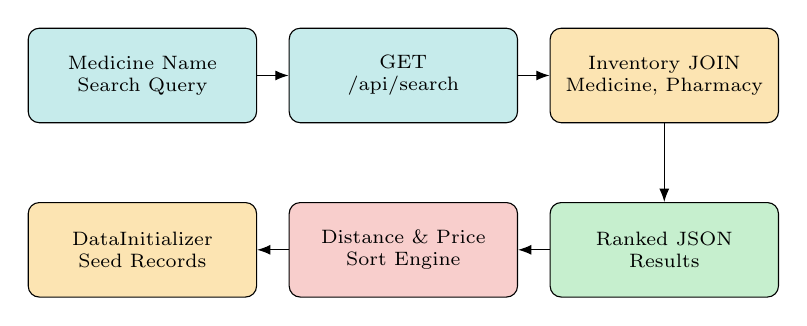
\begin{tikzpicture}[
    node distance=0.4cm and 0.4cm,
    box2/.style={rectangle, draw, rounded corners, minimum width=2.9cm, minimum height=1.2cm, align=center, font=\scriptsize},
    >=Latex
]
\node[box2, fill=tealBox] (n1) {Medicine Name\\Search Query};
\node[box2, fill=tealBox, right=of n1] (n2) {GET\\/api/search};
\node[box2, fill=orangeBox, right=of n2] (n3) {Inventory JOIN\\Medicine, Pharmacy};

\node[box2, fill=greenBox, below=1cm of n3] (n4) {Ranked JSON\\Results};
\node[box2, fill=redBox, left=of n4] (n5) {Distance \& Price\\Sort Engine};
\node[box2, fill=orangeBox, left=of n5] (n6) {DataInitializer\\Seed Records};

\draw[->] (n1) -- (n2);
\draw[->] (n2) -- (n3);
\draw[->] (n3) -- (n4);
\draw[->] (n4) -- (n5);
\draw[->] (n5) -- (n6);
\end{tikzpicture}
\caption{Core Search and Inventory Query Pipeline}
\end{figure}

\begin{itemize}
    \item \textbf{Medicine entity/repository} -- stores medicine name and description (e.g., Paracetamol, Ibuprofen).
    \item \textbf{Pharmacy entity/repository} -- stores pharmacy name, address/area, and latitude/longitude used for distance calculations.
    \item \textbf{Inventory entity/repository} -- links a Medicine to a Pharmacy with price, stock quantity, and a last-updated indicator, and is the table actually queried for availability.
    \item \textbf{REST endpoints} -- \texttt{GET /api/medicine} and \texttt{GET /api/pharmacy} expose the base catalogues, while \texttt{GET /api/search?medicine=\{name\}} returns matching inventory records for a given medicine name.
    \item \textbf{DataInitializer} -- seeds the database with sample medicines, pharmacies, and inventory records on first run, which was used to validate the schema and endpoints end-to-end.
\end{itemize}

\subsection{Module 2: Secondary Features}

Building on the core module, the following features extend MedFinder toward its full proposed scope. Figure 2.3 shows how a search result flows into filtering and reservation.

\begin{figure}[h!]
\centering
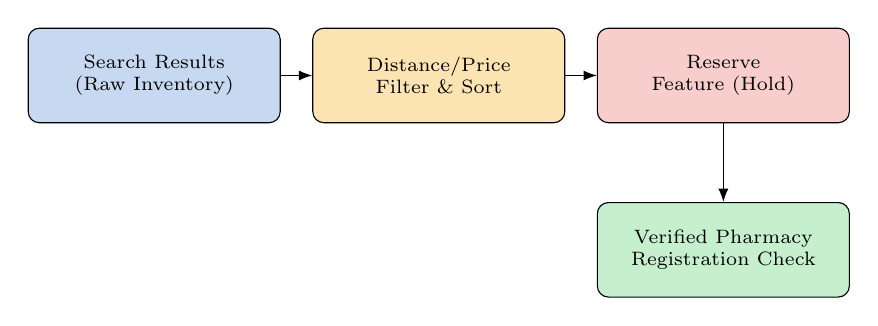
\begin{tikzpicture}[
    node distance=0.4cm and 0.4cm,
    box2/.style={rectangle, draw, rounded corners, minimum width=3.2cm, minimum height=1.2cm, align=center, font=\scriptsize},
    >=Latex
]
\node[box2, fill=blueBox] (m1) {Search Results\\(Raw Inventory)};
\node[box2, fill=orangeBox, right=of m1] (m2) {Distance/Price\\Filter \& Sort};
\node[box2, fill=redBox, right=of m2] (m3) {Reserve\\Feature (Hold)};
\node[box2, fill=greenBox, below=1cm of m3] (m4) {Verified Pharmacy\\Registration Check};

\draw[->] (m1) -- (m2);
\draw[->] (m2) -- (m3);
\draw[->] (m3) -- (m4);
\end{tikzpicture}
\caption{Secondary Feature Flow: Filtering, Reservation, and Verification}
\end{figure}

\begin{itemize}
    \item \textbf{Distance and price filtering/sorting} of search results, so users can prioritise the nearest or cheapest available option.
    \item \textbf{Reserve feature} allowing a user to place a temporary hold on an in-stock item at a chosen pharmacy until they arrive.
    \item \textbf{Verified pharmacy registration}, so only recognised, authentic stores can be listed and appear in search results.
    \item \textbf{Planned refinements} such as fuzzy text matching on medicine names (to tolerate spelling variants) and periodic inventory refresh to keep stock counts current.
\end{itemize}

% ============================================================
% CHAPTER 3: RESULTS AND EVALUATION
% ============================================================
\chapter{Results and Evaluation}

\section{Testing Methodology}

The backend was tested incrementally, endpoint by endpoint, directly through the browser and by inspecting the underlying MySQL tables in phpMyAdmin. Each endpoint (\texttt{/api/medicine}, \texttt{/api/pharmacy}, \texttt{/api/search}) was checked in isolation to confirm it returned the expected JSON before moving on to the next, which made it straightforward to localise issues -- for example, an empty result from \texttt{/api/search} was traced back to missing rows in the pharmacy and inventory tables rather than a code defect.

\begin{figure}[h!]
\centering
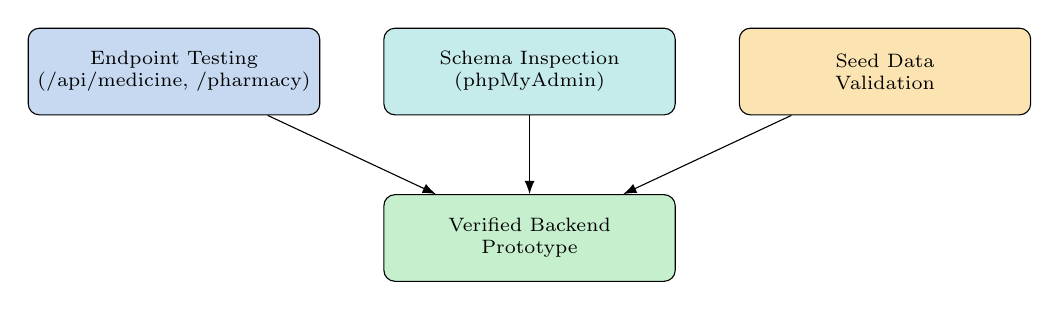
\begin{tikzpicture}[
    box3/.style={rectangle, draw, rounded corners, minimum width=3.7cm, minimum height=1.1cm, align=center, font=\scriptsize},
    >=Latex
]
\node[box3, fill=blueBox] (t1) {Endpoint Testing\\(/api/medicine, /pharmacy)};
\node[box3, fill=tealBox, right=0.8cm of t1] (t2) {Schema Inspection\\(phpMyAdmin)};
\node[box3, fill=orangeBox, right=0.8cm of t2] (t3) {Seed Data\\Validation};

\node[box3, fill=greenBox, below=1cm of t2] (t4) {Verified Backend\\Prototype};

\draw[->] (t1) -- (t4);
\draw[->] (t2) -- (t4);
\draw[->] (t3) -- (t4);
\end{tikzpicture}
\caption{Incremental Endpoint Testing and Schema Validation Framework}
\end{figure}

This process also surfaced and resolved a schema-level issue during development: an existing medicine table had been created without \texttt{AUTO\_INCREMENT} on its \texttt{id} column, which caused insert failures once Hibernate attempted to generate IDs automatically. The fix was to drop the affected prototype tables and allow Hibernate to recreate them with the correct schema, after which seeding and querying worked as expected.

\section{Performance Metrics}

Formal performance testing (load testing, response-time benchmarking, and search-accuracy measurement against a larger dataset) has not yet been carried out on the prototype and is planned as a next step once the frontend is complete and a larger sample dataset is loaded. Table 3.1 summarises the metrics intended to be captured, along with their current status.

\begin{table}[h!]
\centering
\small
\begin{tabular}{p{6.2cm}p{4cm}p{2.8cm}}
\toprule
\textbf{Evaluation Metric} & \textbf{Target Specification} & \textbf{Status} \\
\midrule
Average API response time for /api/search (typical \& peak load) & $\leq$ 500 ms & Pending \\
Accuracy of medicine-name matching (incl. spelling variants) & $\geq$ 90.0\% & Pending \\
Correctness of distance-based ranking vs.\ known coordinates & 100\% & Pending \\
System behaviour as pharmacy/inventory records scale up & Stable throughput & Pending \\
\bottomrule
\end{tabular}
\caption{MedFinder Planned Performance Evaluation Metrics}
\end{table}

\section{Analysis}

At the current stage, the backend prototype reliably exposes medicine, pharmacy, and inventory data through REST endpoints, and the search endpoint correctly returns matching inventory once the database is seeded correctly. This confirms that the core data model and query logic are sound. The main remaining work is integrating a complete frontend against these endpoints, implementing the Reserve and verification features fully, and then subjecting the combined system to the performance and accuracy testing described above.

% ============================================================
% CHAPTER 4: CONCLUSION
% ============================================================
\chapter{Conclusion}

\section{Summary of Work}

This project set out to build MedFinder, a web application that lets patients search for a medicine and instantly see which nearby, verified pharmacies have it in stock, along with price and distance. A three-tier architecture was designed with a Spring Boot REST API and a MySQL database, and a working backend prototype was implemented covering the Medicine, Pharmacy, and Inventory data model, seed data, and the core search endpoint, with the schema and endpoints validated through direct testing.

\section{Key Findings}

\begin{itemize}
    \item A relational schema of Medicine, Pharmacy, and Inventory tables is sufficient to model real-time, store-level availability and supports the search-by-medicine query pattern MedFinder needs.
    \item Spring Boot with Spring Data JPA and Hibernate allows the core API to be built and iterated on quickly, though schema-generation details (such as \texttt{AUTO\_INCREMENT} columns) need care when the database already contains tables from earlier iterations.
    \item Testing endpoints incrementally, and inspecting the database directly, was an effective way to isolate issues between the application layer and the data layer.
\end{itemize}

\section{Future Work and Recommendations}

For the final project phase, the team will implement:

\begin{itemize}
    \item Complete the frontend so users can search, filter by distance/price, and reserve medicine through a full interface rather than raw API calls.
    \item Implement the pharmacy verification/registration workflow so only recognised stores can list inventory.
    \item Add fuzzy/approximate text matching on medicine names to make search more forgiving of typos and brand-name variants \cite{ref2}.
    \item Introduce a mechanism for pharmacies to keep inventory data current (manual updates initially, with API-based or automated sync as a longer-term goal).
    \item Carry out the performance and accuracy evaluation outlined in Section 3.2 once the system is feature-complete.
    \item Consider CI/CD automation and basic scalability planning (e.g., indexing, caching) before any pilot deployment beyond a single city \cite{ref1}.
\end{itemize}

\section{Final Remarks}

MedFinder addresses a genuine and common problem -- not knowing, in advance, which nearby pharmacy actually has a needed medicine in stock. The prototype work completed so far demonstrates that the core idea is technically workable: a searchable, store-level inventory system can be built on a conventional and well-supported stack. The remaining work is primarily one of completing the user-facing features and validating the system's accuracy and performance at a realistic scale.

\end{document}